 

\chapter{Previous Introduction}



In the Internet, network providers and content delivery providers are often distinct entities. 
This is a reason why people tend to view networking and content delivery as independent disciplines. 

%Yet, both networks and content delivery systems contribute towards the common goal of improving user-perceived performance in the Internet. Networks make decisions of capacity planning and traffic engineering to keep the network running free of congestion.  Similarly, content delivery systems use several mechanisms such as such as content caching, load balancing, and path and protocol optimizations to optimize user-experience.
% do so via several mechanisms such as such as content caching, load balancing, and path and protocol optimizations.

%When a user access a website on the Internet that is serviced by a content delivery network (CDN), the performance it experiences depends on several mechanisms employed by the CDN such as content caching, load balancing, and path and protocol optimizations. A content delivery system also relies on connectivity provided by the underlying network to reach the end-users. Therefore, how the underlying network routes traffic also contributes towards user-perceived performance. While both networking and content delivery share a common goal in improving user-perceived performance, people tend to view them as independent disciplines. 
%People hold this viewpoint because content delivery systems and networks are often under the control of distinct, non-cooperating entities in the Internet.

In recent times, a few prominent efforts have brought networking and content delivery under a single umbrella. Some of these works are network architecture proposals such as DONA \cite{DONA}, ICN \cite{Ghodsi} ,  and the most prominent, content-centric Networking (CCN) \cite{CCN}, which has presented a complete redesign of the Internet protocols to reflect content delivery goals. 
While today's Internet protocols are designed to provide host-to-host communications, these architectures treat content as first-class network entities, and enable direct communication between users and the content they are interested in.
%Users can register content in the network by its name, and request content registered by other users from the network. 
These architectures obviate  application-layer content delivery systems, as the network layer itself supports content delivery features.
% is a functionality provided by the network itself, instead of an application running as a distributed, overlay service.

A second category of work has developed cooperative strategies for networks and content delivery systems \cite{P4P, JohariGameTheory, CATE}. These cooperative mechanisms are possible because networks' decisions such as routing, and content delivery systems' decisions, such as server selection, affect each others cost and performance objectives. These works have shown that there is potential for leveraging the interaction between networks and content delivery systems to help the objectives of both these entities. 

%A noteworthy example is content-centric networking  proposal on Internet architecture, which has presented a complete redesign of the Internet protocols to reflect content delivery goals.   Another category of work has investigated cooperative strategies for Internet service providers and content providers, and shown that cooperative mechanisms can benefits cost and performance objectives of both these entities  \cite{,,,}.  These examples show two ways in which networks and content delivery systems can benefit each other. First,  network architecture can offer services for streamlining content delivery in the Internet. Second, networks and content delivery systems can use strategies that leverage the interaction between them to help the objectives of both these entities. 


%These works indicate that there are potential benefits to be had by leveraging the interactions between networks and content delivery systems. 

%As these examples show, networks and  content delivery systems influence each other in following ways:
%\begin{itemize}
%\item
%Work on network architectures is often motivated by the goal of streamlining aspects of content delivery in the Internet.
%%The design of content delivery systems depends on what services the underlying network offers, and therefore, work on network architectures often focuses on providing services that are useful in designing content delivery systems.
%\item
%Content delivery systems and networks both shape the flow of traffic with their respective techniques,  and these techniques react to changes in the flow of traffic. As a result, content delivery systems and networks affect each other's decisions. 
%\end{itemize}

In this thesis, we share the vision of studying networking and content delivery as inter-dependent disciplines. Towards this vision, we present research both in network architectures and on network-content delivery interactions. 

%\textbf{Network support for content delivery to mobile end-hosts:}  
While content-centric architectures enhance content delivery, they face similar challenges as the current Internet  in handling end host mobility in a seamless manner. 
Some communication patterns are intrinsically host-to-host, e.g., VoIP calls, and hence require initiating and maintaining connections to mobile end-hosts.
Making content as first-class network entities helps little in solving this problem compared to the current Internet which provides host-to-host communication. 
To seamlessly support for mobility both in current Internet and other network architectures, we believe that a key enabling technology is a global name service which translates host names to their network addresses under frequent mobility of end-hosts.
%Our position is that seamless support for mobility, both in current Internet and in other network architectures, requires a global name resolution service for mapping names of end-hosts to their network address under frequent mobility.


%The current name service, Domain Name System (DNS), is ill-equipped to provide name resolution to mobile hosts due to its heavy reliance on TTL-based caching and scalability concerns associated with high update rates of mobile hosts.The contribution of this thesis is the design and implementation of a scalable, geo-distributed name service to handle the demands of a highly mobile workload. Further, our name service design is flexible to provide name resolution in present day Internet as well as several proposed network architectures, and therefore addresses the end-host mobility problem across many of them.



%
%While content-centric architectures provide natural support for many communication patterns, some communication patterns do require host-to-host communications, e.g., VoIP calls. 
%These communication must deal with mobility of end-hosts, and frequently break down in the face of end-host mobility. 


%Content-centric architecture do not make it easier to support host-to-host communications, 
%
%It is no easier to support host-to-host communications in these architectures than in the Internet. 
%
%host-to-host communications break down in the face of end-host mobility. 
%
%Content-centric network
%
% some aspects of content delivery, they help little in addressing the problems resulting from end-host mobility of end-hosts. Mobility of an end-hosts disrupts data transfers destined to it, and 



%\textbf{Network support for content delivery to mobile end-hosts:}  A key problem in today's Internet, identified and addressed by many network architectures, is the lack of support of mobility of end-hosts.Despite several efforts, initiating and maintaining seamless connections to mobile end-hosts has remained an elusive goal.Our position is that Internet's lack of support for end-host mobility is not because of Internet's IP-based routing, or the naming structure used by end-hosts. The problem lies in the design of the name resolution service for mapping host names to their network address.  The current name service, Domain Name System (DNS), is ill-equipped to provide name resolution to mobile hosts due to its heavy reliance on TTL-based caching and scalability concerns associated with high update rates of mobile hosts. The contribution of this thesis is the design and implementation of a scalable, geo-distributed name service to handle the demands of a highly mobile workload. Further, our name service design is flexible to provide name resolution in present day Internet as well as several proposed network architectures, and therefore addresses the end-host mobility problem across many of them.

%\textbf{Network-content delivery interactions:}  
We find that research on network and content delivery interactions has paid little attention to the role of content placement strategies, i.e., the locations at which a content is placed in the network.  For example, \cite{Roughgarden,selfishQiu} study the interaction of selfish overlay routing and network routing, and \cite{P4P, JohariGameTheory, CATE} study the interaction of server selection policies and network routing. 
However, content placement is a key factor affecting the performance and cost of content delivery. Content placement also shapes the flow of traffic in a network and therefore interacts with network routing strategies. Thus, content placement strategies must be taken into account while studying this interaction.

\section{Thesis goals}

The main goals of this thesis are the following:

\begin{itemize}
\item
Evaluate how content placement strategies affect the objectives of networks and content delivery systems, while accounting for  the interaction of network and content delivery.
\item
Design, implement and evaluate a scalable name service that provides name to network address resolution for mobile hosts in the Internet as well as other network architectures that require name-to-address resolution.
\end{itemize}

%Our contribution is the design and implementation of a scalable, geo-distributed name service to handle the demands of a highly mobile workload. Further, our name service design is flexible to provide name resolution in present day Internet as well as several proposed network architectures, and therefore addresses the end-host mobility problem across many of them.

%In this thesis, we consider the interaction between networks and content delivery systems in three problem domains and ask which placement strategies are effective in improving the objectives of networks and content delivery systems.  Further, we investigate the relative importance of  placement decisions vs network routing decisions. Our contributions are to show that (1) simple placement strategies can improve performance-, cost-, and energy-objectives of networks and content delivery systems, and (2)  content placement plays a greater role than network routing decisions in achieving these objectives.

%Our position if that building support for end-host mobility has remained an elusive goal because of a lack of global name resolution infrastructure for . 
%Internet routing, naming 
%Despite of 
%
% 
%As a result, content delivery systems need to work around the problem of being unable to initiate and maintain connections to mobile hosts by building application-level mechanisms such as push notification services.
%
%The problem lies in the name resolution infrastructure, 
%
%We believe Internet Our position is that building support for end-host mobility 
% 
%\textbf{Network support for content delivery to mobile end-hosts:} 
%%Second, we enhance network architecture support for content delivery to mobile end-hosts.
%A key problem in today's Internet, identified by many, is the lack of support of mobility of end-hosts.
%As a result, content delivery systems need to work around the problem of being unable to initiate and maintain connections to mobile hosts by building application-level mechanisms such as push notification services. A promising approach to solve this problem, as proposed by several architectures, is via a global name resolution service that translates host names to their network address under frequent  mobility of end-hosts. 
%Despite several proposals to handle end-host mobility, attaining mobility in the Internet has remained an elusive goal. 
%As a result, content delivery systems need to work around the problem of being unable to initiate and maintain connections to mobile hosts by building application-level mechanisms such as push notification services. A promising approach to solve this problem, as proposed by several architectures, is via a global name resolution service that translates host names to their network address under frequent  mobility of end-hosts. 
%


%However, the name service of  the Internet,  Domain Name System (DNS), is ill-equipped to provide name resolution to mobile hosts due to its heavy reliance on TTL-based caching and scalability concerns associated with high update rates of mobile hosts. Our contribution is the design, implementation, and evaluation of Auspice, a scalable, geo-distributed name service for mobile hosts.  

%A key decision for this service, affecting both performance and update costs, is the placement of name records of mobile hosts. Auspice infers pockets of high demand for a name and uses a heuristic placement scheme to provide low address lookup latency, low update cost, and high availability. Our evaluation of Auspice's implementation  shows that Auspice significantly outperforms both commercial managed DNS services as well as DHT-based replication alternatives to DNS.

\eat{
***************************v1**************************

When a user access a website on the Internet that is serviced by a content delivery network (CDN), the performance it experiences depends on several mechanisms employed by the CDN such as content caching, load balancing, and path and protocol optimizations. A content delivery system also relies on connectivity provided by the underlying network to reach the end-users. 
Therefore, how the underlying network routes traffic also contributes towards user-perceived performance.
While both networking and content delivery share a common goal in improving user-perceived performance, people tend to view them as independent disciplines. 
%People hold this viewpoint because content delivery systems and networks are often under the control of distinct, non-cooperating entities in the Internet.

In recent times, a few prominent efforts have brought networking and content delivery under a single umbrella. A noteworthy example is content-centric networking  proposal on Internet architecture \cite{,}, which has presented a complete redesign of the Internet protocols to reflect content delivery goals.  Another category of work has investigated cooperative strategies for Internet service providers and content providers, and shown that cooperative mechanisms can benefits cost and performance objectives of both these entities  \cite{,,,}.  
These examples show two ways in which networks and content delivery systems can benefit each other. First,  network architecture can offer services for streamlining content delivery in the Internet. Second, networks and content delivery systems can use strategies that leverage the interaction between them to help the objectives of both these entities. 


%These works indicate that there are potential benefits to be had by leveraging the interactions between networks and content delivery systems. 

%As these examples show, networks and  content delivery systems influence each other in following ways:
%\begin{itemize}
%\item
%Work on network architectures is often motivated by the goal of streamlining aspects of content delivery in the Internet.
%%The design of content delivery systems depends on what services the underlying network offers, and therefore, work on network architectures often focuses on providing services that are useful in designing content delivery systems.
%\item
%Content delivery systems and networks both shape the flow of traffic with their respective techniques,  and these techniques react to changes in the flow of traffic. As a result, content delivery systems and networks affect each other's decisions. 
%\end{itemize}


%We elaborate on these contributions below.

%The goals of this thesis are to enhance 

We share the vision of studying networking and content delivery as inter-dependent disciplines. Towards this vision, we present research on two topics: 

\emph{Role on placement on network and content delivery interactions:}  
%First, we shed light on the interaction of networks and content delivery systems focusing on the role of placement strategies. 
Content placement, i.e., the locations at which a content is placed in the network, is a key factor in shaping the flow of traffic in a network, e.g., placing content at a large number of locations results in localized traffic flows. Yet, research on network and content delivery interactions has paid little attention to the role of content placement strategies, e.g., \cite{a,b,c} study the interaction of selfish overlay routing and network routing, and \cite{a,b,c} study the interaction of server selection policies and network routing. We consider the interaction between networks and content delivery systems in three problem domains and ask which placement strategies are effective in improving the objectives of networks and content delivery systems.  Further, we investigate the relative importance of  placement decisions vs those of other decisions such as routing and server selection. Our contributions are to show that (1) simple placement strategies can improve performance-, cost-, and energy-objectives of networks and content delivery systems, and (2)  content placement plays a greater role than decisions of routing or server selection in achieving these objectives.


 %\emph{Role of content placement strategies:} 
 
\emph{Network architecture support for content delivery to mobile end-hosts:}
%Second, we enhance network architecture support for content delivery to mobile end-hosts.  
Today, content delivery systems need to work around the problem of being unable to initiate and maintain connections to mobile hosts by building application-level mechanisms such as push notification services. A promising approach to solve this problem, as proposed by several architectures, is via a global name resolution service that translates host names to their network address under frequent  mobility of end-hosts. However, the name service of  the Internet,  Domain Name System (DNS), is ill-equipped to provide name resolution to mobile hosts due to its heavy reliance on TTL-based caching and scalability concerns associated with high update rates of mobile hosts. Our contribution is the design, implementation, and evaluation of Auspice, a scalable, geo-distributed name service for mobile hosts.  A key decision for this service, affecting both performance and update costs, is the placement of name records of mobile hosts. Auspice infers pockets of high demand for a name and uses a heuristic placement scheme to provide low address lookup latency, low update cost, and high availability. Our evaluation of Auspice's implementation  shows that Auspice significantly outperforms both commercial managed DNS services as well as DHT-based replication alternatives to DNS.
}
%Several network architectures have proposed improving support for end-host mobility 



%The contributions of this thesis are in understanding the interactions of networks and content delivery systems, and in enhancing network architecture to support content delivery to mobile end-hosts. 
% is in area of network architectures, in particular, towards support for end-host mobility, as well as  in .

%This goals of this thesis are to shed light on the role of placement strategies on the interaction of networks and content delivery systems and to enhance the network architecture support for end-host mobility so that content delivery systems can support rich communication patterns e.g., mobile-to-mobile data transfer, server-to-mobile push notifications, without building application-level mechanisms to do so.

%Our goal is to enhance and leverage the interactions between networks and content delivery systems towards improving user-perceived performance. To this end, we address the following problems:
%We seek to leverage and enhance the interactions between networks and content delivery systems. 


 % A key contribution of our work is to show that simple placement strategies are effective in improving cost-,performance-, and energy-related metrics for networks and content delivery systems. 

%\emph{Network support for end-host mobility:} 
%one of the long challenges which work in network architecture has tried to address is support of end-host mobility.
%1. today, content delivery suffers because of that
%2. a promising approach alluded to by several architectures is  a global name resolution infrastructure, which coupled with end-to-end approach could bring to the goal of seamless mobility. 
%3. current dns not the solution, because of high update load, and TTL caching.
%4. distributed systems challenge of scalable, high update rates.
%Today, content delivery systems need to work around the problem of being unable to initiate and maintain connections to mobile hosts by building application-level mechanisms such as push notification services. Our position is that end-host mobility can be seamlessly handled with the support of a global name service that translates host names to their network address under frequent  mobility of end-hosts.  To this end, we present the design, implementation, and evaluation of Auspice, a scalable, geo-distributed name service.  A key decision for this service, affecting both performance and update costs, is the placement of name records of mobile hosts. Auspice infers pockets of high demand for a name and uses a heuristic placement scheme to provide low address lookup latency, low update cost, and high availability. Our evaluation of Auspice's implementation  shows that Auspice significantly outperforms both commercial managed DNS services as well as DHT-based replication alternatives to DNS.

%We elaborate on both these research topics in the rest of this chapter.


\section{Network and content delivery interactions}

Section 1.1.1 explains why understanding network and content delivery interactions is a key research problem for both these areas. 
Section 1.1.2 explains the role of content placement in network-content delivery interactions by showing how it affects both network and content delivery objectives. 
Section 1.1.3 describes how network and content delivery interact in three scenarios considered in this thesis--an ISP network, a network CDN, and a CDN datacenter--and the research questions we address in each of them.

%We start by explaining why content placement affects objectives of not only content delivery but networks as well. This section   First, we consider the interaction between an Internet service provider's traffic engineering and location diversity of content created by an (independent) content delivery system. Second, we consider a network CDN, i.e., an Internet service provider offering content delivery to its users through its network, which is seeking to optimize cost/performance objectives under resource constraints. Third, we consider a content-serving data center seeking to minimize its energy use.  
%The latter two problems consider scenarios where network and content delivery are under the control of a single entity, which opens up the possibility of joint optimization of network and content delivery. 

 
%This section explain how content placement affects both network and content delivery objectives and  describe the three problem domains where we study network and content delivery interactions.

\subsection{Why networks and content delivery interactions matter?}
We believe that studying network and content delivery interactions is important for two reasons: 
\begin{itemize}
\item
\textbf{Re-evaluate known results:} Network routing (a.k.a. traffic engineering)  and content delivery  strategies have evaluated independent of one another. Therefore, it is necessary to re-evaluate existing traffic engineering and content delivery strategies taking into account the interaction between them.
\item
\textbf{Design new approaches:} In scenarios where networks and content delivery systems cooperate with each other, we can leverage these interactions to design new approaches for improving traffic engineering and content delivery objectives.
\end{itemize}

%
%- performance needs to be reevaluated 
%- potential to leverage these interactions to improve network 

\subsection{Placement affects networks and content delivery systems}

Content placement strategies play a major role in deciding user-perceived performance and costs of content delivery. When placement strategies replicate content, they improve user-perceived performance but increase costs of a content delivery system, e.g., replicating a large video file increases the storage requirements, replicating dynamic objects increases the cost of propagating updates to all locations.  Content placement strategies help reduce costs of replicating content, while improving user-perceived performance. Placement strategies exploit geographic and temporal locality of requests seen in real-world workloads\cite{NCDN,youtubeUGC,vodP2Pbenefit,cellularvideotraffic}. They replicate content at those times and and at those locations where the content is more popular, and thereby help optimize performance while minimizing replication costs.

Content placement strategies interact with traffic engineering and affect network objectives as shown by the following example. Consider the network in Figure \ref{fig:NetworkExample} whose objective is to minimize the maximum link utilization (MLU). Node $C$ has an object in its cache that is requested by end-users at nodes $A$ and $D$. Suppose that one unit of traffic needs to be routed from $C$ to $A$ and $0.5$ units  from $C$ to $D$ to satisfy the demand for that object. The routing that serves the demanded object while minimizing the MLU is shown in the figure. 
Note that the routing that achieves the MLU of 0.5 is not possible with a shortest path routing as that would route all the traffic demand from $C$ to $A$ via $B$ or $D$, resulting in an MLU of 1. Thus, a routing protocol which splits flows along multiple paths is necessary to achieve an MLU of 0.5.

Suppose that there is some space left in the content server's cache at node $B$ to accommodate an additional copy of the demanded object. By creating an additional copy of the object at $B$, the traffic demand of $A$ can be satisfied from $B$ and the demand of $D$ from $C$ achieving the an MLU of $0.125$. In this case, judicious content placement decreased the MLU by a factor of $4$.  Even more interestingly, this best MLU can be achieved using a shortest path routing scheme. Although this is clearly a ``toy'' example, it illustrates the sophisticated interaction between content placement and routing and potential opportunities for networks to reduce costs via effective placement strategies.


%NetworkExample
\begin{figure}
\centerline{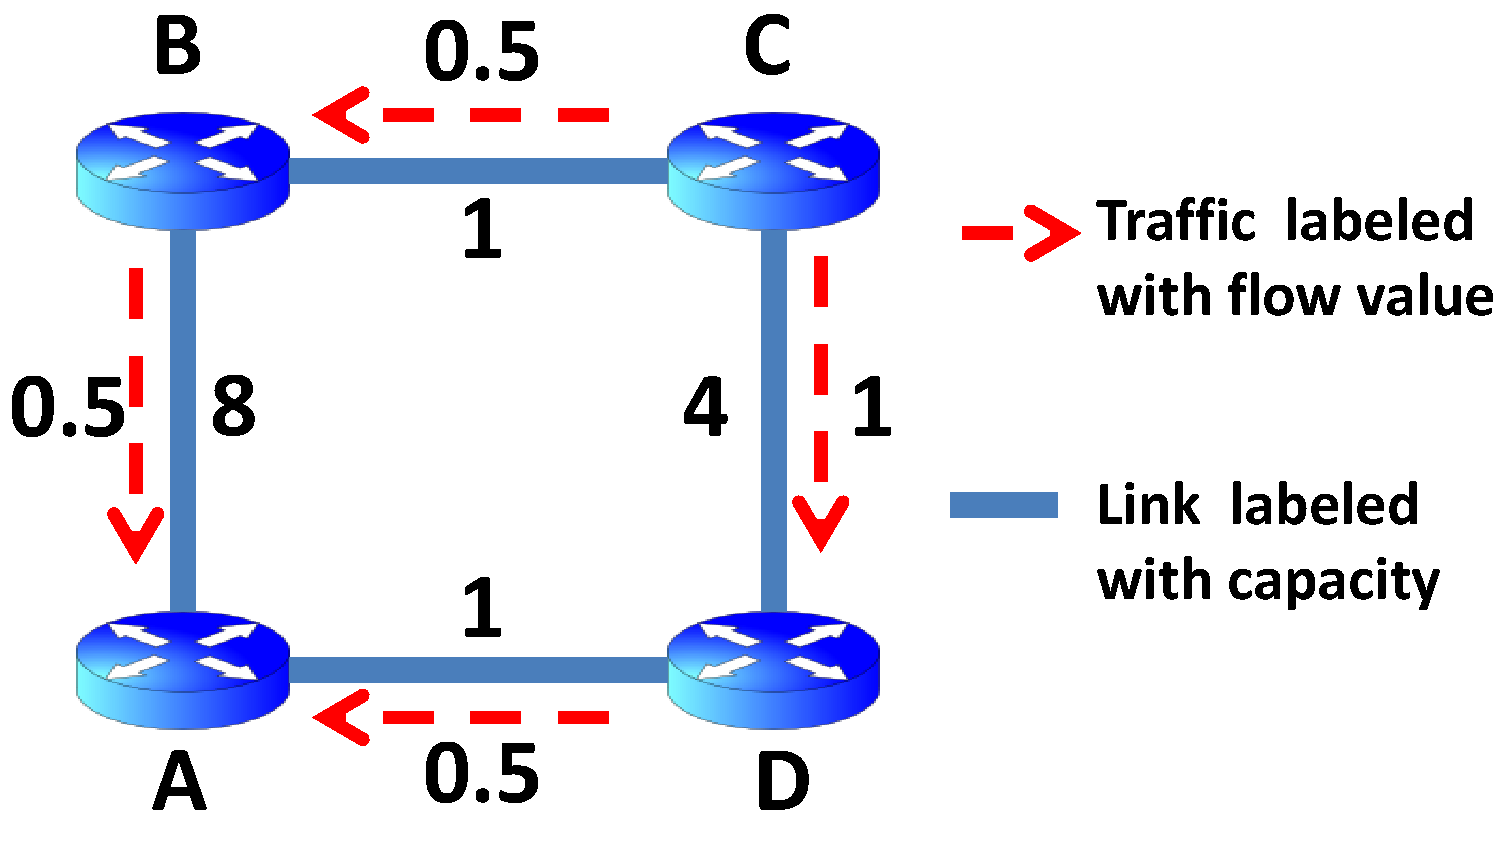
\includegraphics[height=1.2in]{ncdnpaper/ncdn-example}}\vspace*{-0.1in}
\caption{Interaction of placement and routing}
\vspace*{-0.2in}
\label{fig:NetworkExample}
\end{figure}



%
%\section{Role of content placement strategies}
%
%%We study the interaction of networks and content delivery across three problem domains. First, we consider an Internet service provider network and show 
%
%\subsection{Placement affects network and content delivery objectives}
%
%
%
%Placement affects content delivery objectives.
%
%Placement affect network objectives and routing decisions. 

%In Section 1.1.2-1.1.4, we give specific examples of placement strategies, and their interaction with routing strategies from the problems we present in this thesis.


\subsection{Research problems}

\subsubsection{ISP network with location diversity of content}

The first problem (described in Chapter 3) studies the interaction of ISP traffic engineering with content delivery in a network with location diversity of content. 
We seek to understand how this interaction affects traffic engineering (TE) metrics, as well as user-perceived metrics, such as file download time, and VoIP call quality.
We consider several classes of TE schemes, and networks with varying location diversity of content. 
In all cases, applications leverage location diversity of content by downloading in parallel from all locations.
We consider a simple placement scheme that replicates content at random locations, and conduct very large scale experiments simulating ISP traffic as a collection of TCP flows seeking to answer following questions:
\begin{itemize}
\item
How does the user-perceived performance depend on which TE strategy is used?
\item
What is the effective capacity of different TE strategies to tolerate surges in traffic demand?
\item
How much benefit does TE give over a simple static routing?
\end{itemize}



%This problem studies the interaction of ISP traffic engineering and location diversity of content in the network created by content delivery systems. An ISP uses traffic engineering for avoiding congestion hotspots and increasing  the effective capacity of the network. On the other hand, content delivery systems create location diversity of content in the network by replicating content, enabling applications to leverage the location diversity by downloading in parallel from multiple locations.  As applications adapt to location diversity of content, they change link utilizations and affect the result of ISP traffic engineering. Conversely, traffic engineering computes the network-level routes and affects how an application will split its traffic among multiple locations. We consider a simple placement policy of replicating content a small number of random locations, and seek to answer following questions while accounting for the effect of location diversity of content:
%, considering the interaction of route optimization and application adaptation to location diversity: 




\subsubsection{Network CDN}

The second problem (described in Chapter 4) studies network and content delivery interactions in a network CDN (NCDN), where a single entity makes both traffic engineering and content delivery decisions.
We seek to find the best way for an NCDN to leverage this interaction for optimizing both TE metrics and content delivery metrics.
We consider a wide-range of strategies for an NCDN including (1) joint optimization of traffic engineering, placement, and request redirection based on historic demand patterns (2) simple unplanned approaches for traffic engineering and  content placement (3) ideal joint optimization strategy with perfect future knowledge of demand patterns. 
We conduct trace-driven evaluations based on real network topologies and content access traces of millions of users from the world's largest CDN, Akamai, to answer following questions:
\begin{itemize}
%\item
%How should an \ncp\ jointly optimize content placement, routing, and request redirection decisions so as to optimize TE metrics and user-perceived latency?
\item
How much benefit do joint optimization strategies yield over simpler strategies as practiced today, and does the benefit warrant the added complexity?  
\item
How do \planned\ strategies (i.e., using knowledge of recently observed demand patterns or hints about anticipated future demands) for placement and routing compare against simpler, \unplanned\ strategies?
\item
What is the relative importance of optimizing placement vs optimizing routing?
\end{itemize}


%An Internet service provider offering content delivery to its users through its network is called a network CDN (NCDN). An NCDN is a unique form of CDN that controls both the content delivery as well as the underlying network. 
%An NCDN  can potentially leverage the interaction between content delivery and routing in the best-possible manner by jointly optimizing both these decisions. 
%The intriguing prospect of jointly optimizing content delivery and routing raises several research questions that we seek answers to:

%\begin{itemize}
%\item
%How should an \ncp\ determine content placement, network routing, and request redirection decisions so as to optimize network cost and user-perceived latency? 
%\item
%How much benefit do joint optimization strategies yield over simpler strategies as practiced today, and does the benefit warrant the added complexity?  
%%\item
%%How do content demand patterns and placement strategies impact network cost?  
%\item
%How do \planned\ strategies (i.e., using knowledge of recently observed demand patterns or hints about anticipated future demands) for placement and routing compare against simpler, \unplanned\ strategies?
%\end{itemize}

\subsubsection{Energy-efficient CDN datacenter}

The third problem (described in Chapter 5) considers the design of an energy-efficient CDN datacenter while ensuring a minimal impact on user-perceived performance either due to cache misses or highly-loaded servers.
In a CDN datacenter, content placement is determined by load balancing and server shutdown policies. 
Thus, placement decisions implicitly affect performance and energy use of a CDN datacenter. 
Prior work in this area has explored independent strategies for reducing energy use of servers and network components in a datacenter. In comparison, we are exploring  a joint optimization of traffic engineering and server shutdown strategies which can help increase datacenter network energy savings.
A key focus of this work is to measure user-perceived metrics such as file download times to investigate the impact of energy minimizing strategies on end-user performance. 
We plan to conduct  trace-driven evaluations with a traces from a commercial CDN datacenter as well as experiments with a prototype to answer following questions:
\begin{itemize}
\item
What is the impact of energy-saving strategies on user-perceived performance? How do we design server shutdown and load-balancing strategies to minimize this impact?
\item
How much additional energy savings can be obtain by a joint optimization of network and server energy?
\item
How do different types of content workloads, e.g, video, downloads, mixture of all traffic types, affect these results?
\end{itemize}
%The third problem (described in Chapter 5) considers network and content delivery interactions in designing an energy-efficient CDN datacenter.Our goal is to design traffic engineering, server shutdown, and load-balancing strategies that maximize energy savings and ensure a minimal impact on user-perceived performance either due to cache misses or highly-loaded servers. To maximize energy savings, we are exploring a joint optimization of traffic engineering and server shutdown strategies.
%Content placement, i.e., the locations at which a content is placed in the network, is a key factor in shaping the flow of traffic in a network, e.g., placing content at a large number of locations results in localized traffic flows. Yet, research on network and content delivery interactions has paid little attention to the role of content placement strategies, e.g., \cite{a,b,c} study the interaction of selfish overlay routing and network routing, and \cite{a,b,c} study the interaction of server selection policies and network routing. We consider the interaction between networks and content delivery systems in three problem domains and ask which placement strategies are effective in improving the objectives of networks and content delivery systems.  Further, we investigate the relative importance of  placement decisions vs those of other decisions such as routing and server selection. 



\section{Network support for end-host mobility}
This section describes why today's Internet needs to provide support to handle end-host mobility, how a global name service helps achieve this goal, and what are the challenges in designing such a service.

Mobile devices dominate the Internet both in number and in the amount of traffic generated, yet Internet lacks the infrastructure support for initiating and maintaing connections to mobile end-hosts.
This limitation poses a problem to mobile app developers who need to use mobile-to-mobile communications or reestablish server-to-mobile communications after a mobility of end-host. 
That app developers need to redundantly develop app-level support to handle end-host mobility is a hindrance for long-term growth and innovation in the Internet.

%How a global name service helps achieve this goal:
%- helps connection establishment:
%- helps mid-connect mobility rapidly:
%- does not increase data path stretch or internet-routing table sizes:

A global name service that translates mobile device name to its network addresses is a key enabler to support end-host mobility in the Internet due to several reasons.
First, a global name service can support connection establishment to a mobile host by returning its current network addresses on an address lookup.
Second, a global name service complements end-to-end connection migration approaches to handle mid-connection mobility of one or both end points in a seamless manner\cite{Migrate,ECCP,TCP-R}.
Third, a global name service handles end-host mobility without inflating the length of the data path or the forwarding table sizes, thereby maintaining the performance and scalability of the Internet.

%What are the key requirements in designing such a service:
%- high update load
%- low lookup latency to authoritative name servers
%- flexibility

There are three main challenges in designing a global name service for mobile hosts: (1) Scalability: The name service must scale to the order of billions of name records to provide name resolution for mobile devices compared to 136M records in current DNS \cite{whois}. (2) High update rates: The name service is expected to encounter a very high loads of updates, tens of updates/day from billions of devices.  (3) Limited cacheability: The name service cannot be expected to take advantage of TTL-based caching as much as DNS does for today's domain names because name records of mobile hosts are expected to become state quickly. As address lookups to the name service is frequent operation, the name service must absorb the additional load of lookups and also provide low address lookup latencies.


%A global name service for mobile hosts must meet some key requirements: 
%(1) Time-to-connect performance: The name service must ensure that address lookups latencies are small so that connections to mobile devices can be established quickly.
%(2) Availability: The design must be resilient to failures of nodes including disasters impacting an entire datacenter or stub network. By consequence, the design must also prevent crippling load hotspots.
%(3) Update cost: The design must ensure low replication cost. A naive way to minimize lookup latencies is to replicate every name record at every available location, however high mobility implies high update rates, so the cost of pushing each update to every replica would be prohibitive.
%(4) Flexibility: The design must be extensible to supporting a rich set of attributes associated with a name and policies for dealing with mobility, multihoming (e.g.,``prefer WiFi to cellular''), etc. The design should be agnostic to how names, addresses, and resolution policies are represented by a future Internet architecture.

\eat{
A global name service that provides name to address resolution for mobile hosts is a part of a three-piece solution to handle mobility of end-hosts. The other two components are: (1) Globally-routable network addresses: We require that to support arbitrary mobility patterns of end-hosts,  the underlying network is able to route traffic to any valid network address in the Internet. (2) Connection-migration library: An end-host library is necessary to update current network address to the name service and to  migrate connections  after one of the end-hosts has changed its network address due to mobility. The global name service, the third component, handles dynamic address updates from end-hosts and  returns current network address for any mobile host registered with the name service.
Our work focuses on the challenge of designing a global name service, while noting that existing work has addressed many challenges in implementing other two components. Several end-host libraries have built support for connection migration and/or dynamic updates to name service\cite{ECCP,Migrate,MPTCP}. Globally-routable network addresses, too, should become a reality in the Internet once IPv6 gains widespread adoption \cite{ipv6Launch,DhamdhereIPv6} making it feasible to assign a unique network address to every end-host. 


There are three main challenges in designing a global name service for mobile hosts: (1) Scalability: The name service must scale to the order of billions of name records to provide name resolution for mobile devices compared to 136M records in current DNS \cite{whois}. (2) High update rates: The name service is expected to encounter a very high loads of updates, tens of updates/day from billions of devices.  (3) Limited cacheability: The name service cannot be expected to take advantage of TTL-based caching as much as DNS does for today's domain names because name records of mobile hosts are expected to become state quickly. As address lookups to the name service is frequent operation, the name service must absorb the additional load of lookups and also provide low address lookup latencies.



%Our key insight is a placement engine for replicating name records. First placement engine is fully distributed with no single bottleneck. Second, controls the number of replicas based on the observed read and write rates to limit update costs. Third, it infers  pockets of high demand for a name so as to create replicas of resolvers for that name close to them and minimizes lookup latency. 

 The key insight in \auspice\ is an engine for automated placement of replicas of name records for a name with low update costs and low latency. \auspice\ achieves low lookup latency by inferring regions of high demand for a name so as to create replicas of records for that name close to those regions. \auspice\ achieves low lookup latency,  low update costs, and high availability across all replica locations using a placement optimization algorithm that (1) controls the number of replicas based on the observed read and write rates, and (2) determines where to place replicas based both on the inferred pockets of demand and the aggregate load at node locations near those pockets. 
}


\section{Contributions}

This section presents a summary of contributions of this thesis. 

\begin{enumerate}
\item
We consider a scheme that places content at a small number of randomly chosen locations in an Internet service provider (ISP) network; end-users leverage the location diversity of content by downloading in parallel from all locations. We compare several route optimization schemes for an ISP accounting for the location diversity of content. Our experiments on real topologies and traffic matrices show that the ability to download content from just 2-4 locations enables all schemes to achieve near-optimal capacity to tolerate surges in traffic demand, and even simple static routing to be within 30\% of optimal. This work was published at IEEE INFOCOM conference held at Shanghai, China in April 2011 with the title \emph{Beyond MLU: an application-centric comparison of traffic engineering schemes}.
\item
We model a single entity that controls both network and content delivery, as in the case of a network CDN (NCDN). An NCDN can independently or jointly optimize both placement and routing. Further, it can make these decisions in ``planned" manner based on recent history of workloads. Our experiments on real network topologies and traces from a large CDN surprisingly show that  ``unplanned'' placement schemes, e.g., LRU caching, combined with a simple static routing outperform (sometimes significantly)  realistic (i.e., history-based) joint-optimization schemes and can achieve network cost and user-perceived latencies close to those of a joint-optimal scheme with future knowledge. This work was published at ACM SIGMETRICS conference held at Pittsburgh, PA, USA  in June 2013 with the title \emph{Distributing content simplifies ISP traffic engineering}.
%\item
%We propose to study energy-minimizing schemes for a CDN datacenter seeking to establish that  significant energy savings are possible with minimal impact on user-perceived performance. Our preliminary results for a CDN datacenter serving on-demand video content show that (1) simple server shutdown and traffic engineering strategies yield close to optimal energy savings (2) energy-saving strategies cause less than 1\% decrease in cache hit rates while using a load-balancing strategy similar to that used by CDNs today.
%We propose to study energy-minimizing schemes for networks seeking to establish that it is feasible to reduce energy consumption for NCDN and datacenter networks. Our central idea is that requests for content can be served by placing content on a subset of nodes during off-peak hours and if these nodes are carefully chosen, it enables large fraction of switches and links to be turned off with a minimal degradation in user-perceived performance. We present preliminary results from trace-driven experiments to support our hypothesis. 
\item
We have designed and implemented a global name service for support name to address resolution for mobile end-hosts. Our name service design, Auspice, infers pockets of high demand for a name and uses a heuristic placement scheme to provide low address lookup latency, low update cost, and high availability.
We have implemented a prototype of Auspice as a geo-distributed key-value store to serve as a flexible name resolution infrastructure for the Internet as well as future Internet architecture proposals.
Our evaluation on multiple testbeds shows that Auspice significantly outperforms both commercial managed DNS services as well as DHT-based replication alternatives to DNS.
%Further, our name service design is flexible to provide name resolution in present day Internet as well as several proposed network architectures, and therefore addresses the end-host mobility problem across many of them.
\end{enumerate}


 
